\begin{table}[H]
\centering
\caption{Síntesis anual del caso base revisado}
{\small\singlespacing\renewcommand{\arraystretch}{1.2}
\begin{tabular}{p{6.1cm}rp{4.5cm}}
\toprule
Indicador & Valor & Unidad o alcance \\
\midrule
Enfriamiento sensible & 59018,63 & kWh térmicos/año \\
Enfriamiento total & 84759,41 & kWh térmicos/año \\
Electricidad de enfriamiento estimada & 45258,71 & kWh eléctricos/año \\
Electricidad de equipos & 39307,57 & kWh eléctricos/año \\
Electricidad de iluminación & 13895,39 & kWh eléctricos/año \\
Ganancia solar por ventanas exteriores & 33884,25 & kWh/año \\
Máximo diario de enfriamiento sensible & 281,52 & kWh/día; 12/03/2025 \\
Temperatura operativa media & 26,53 & $^\circ$C \\
Máxima media diaria operativa & 30,06 & $^\circ$C \\
Días con media operativa mayor de 28 °C & 80 & días; indicador exploratorio \\
Ventilación e infiltración media & 1,68 & renovaciones/hora \\
\bottomrule
\end{tabular}}
\fuente{Elaboración propia a partir de \texttt{Datos Caso Base3.csv}, exportado de la corrida 09 de DesignBuilder. Resultados provisionales.}
\end{table}

La electricidad de enfriamiento es una estimación de DesignBuilder bajo las eficiencias configuradas, no un consumo medido. El enfriamiento total incluye el sensible; ambas magnitudes no se suman. Las temperaturas corresponden a medias del edificio exportadas por el programa.
\clearpage
\begin{table}[H]
\centering
\caption{Resultados mensuales del caso base revisado}
{\small\singlespacing\renewcommand{\arraystretch}{1.2}
\begin{tabular}{lp{2.5cm}p{2.5cm}p{2.2cm}rr}
\toprule
Mes & Electricidad de enfriamiento & Enfriamiento sensible & Solar exterior & $T_{op}$ & $T_{ext}$ \\
\midrule
 & kWh & kWh & kWh & °C & °C \\
Ene & 4758,16 & 5808,86 & 3502,81 & 27,42 & 25,60 \\
Feb & 5091,22 & 6077,35 & 3045,26 & 28,25 & 26,68 \\
Mar & 5898,76 & 7081,25 & 3228,37 & 29,04 & 27,10 \\
Abr & 5362,01 & 6038,52 & 2625,60 & 27,86 & 26,74 \\
May & 5051,05 & 6000,47 & 2428,64 & 27,63 & 25,96 \\
Jun & 3363,42 & 4512,38 & 2269,70 & 26,35 & 24,18 \\
Jul & 2685,92 & 3896,30 & 2247,28 & 25,13 & 23,11 \\
Ago & 2392,37 & 3691,62 & 2388,76 & 25,11 & 22,11 \\
Sep & 2197,24 & 3410,80 & 2480,55 & 24,90 & 21,73 \\
Oct & 2492,05 & 3933,80 & 3023,60 & 25,24 & 22,14 \\
Nov & 2453,15 & 3804,01 & 3244,45 & 25,27 & 22,49 \\
Dic & 3513,36 & 4763,27 & 3399,24 & 26,28 & 23,69 \\
\bottomrule
\end{tabular}}
\fuente{Elaboración propia a partir de \texttt{Datos Caso Base3.csv}, exportado de la corrida 09 de DesignBuilder. Resultados provisionales.}
\end{table}

\begin{figure}[H]
\centering
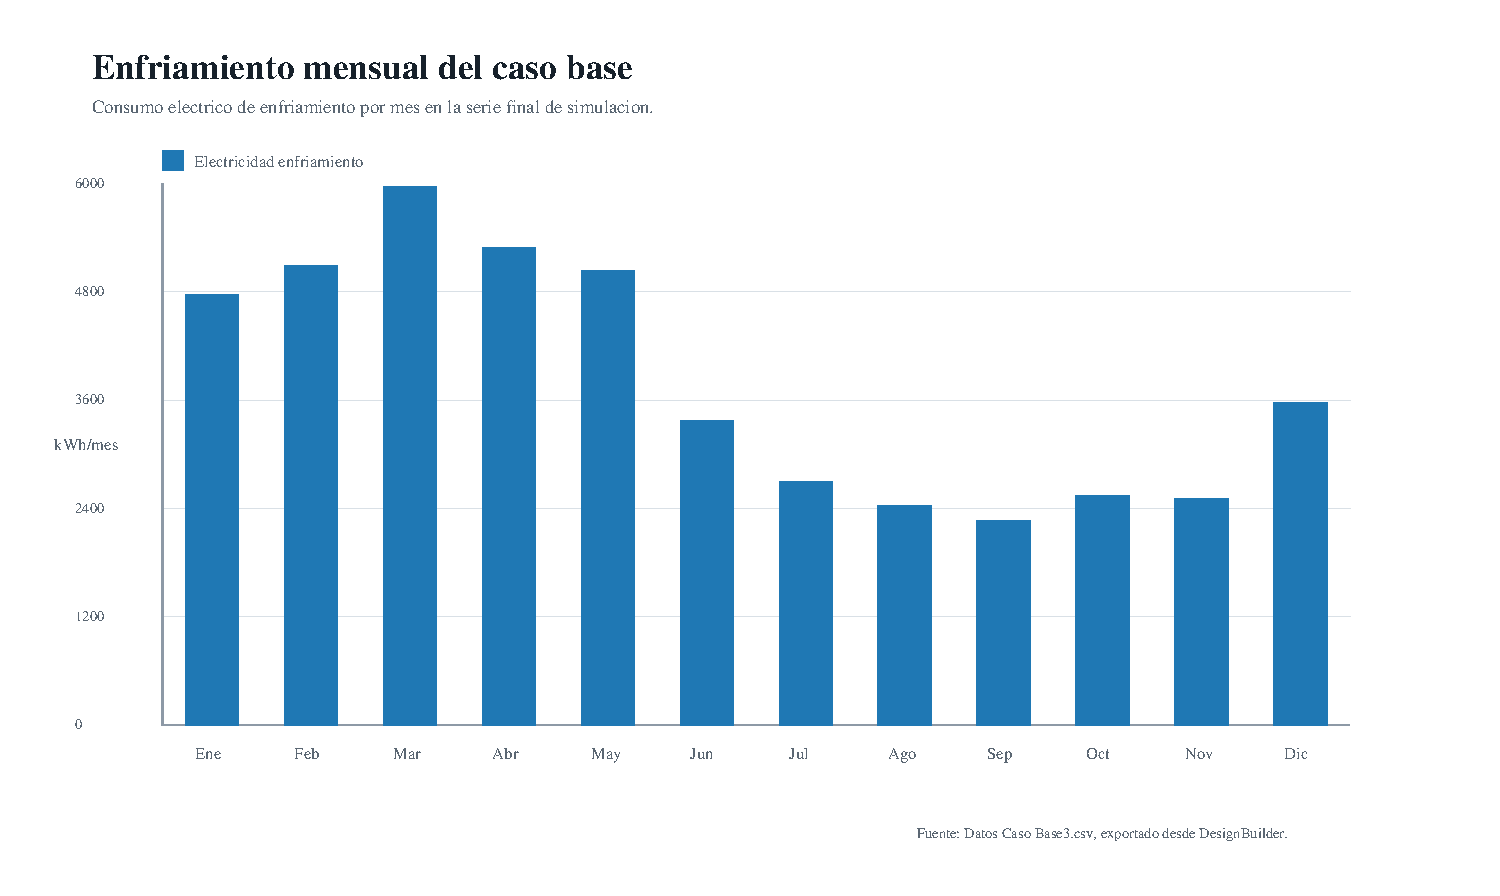
\includegraphics[width=\textwidth]{figuras/caso-base-final-enfriamiento-mensual.pdf}
\caption{Electricidad estimada y energía térmica de enfriamiento por mes}
\fuente{Elaboración propia a partir de \texttt{Datos Caso Base3.csv}, exportado de la corrida 09 de DesignBuilder. Resultados provisionales.}
\end{figure}
\clearpage
\begin{table}[H]
\centering
\caption{Balance térmico anual por componentes del modelo revisado}
{\small\singlespacing\renewcommand{\arraystretch}{1.2}
\begin{tabular}{p{6.2cm}rp{4cm}}
\toprule
Componente & Balance (kWh) & Signo del intercambio \\
\midrule
Misceláneos & 34701,24 & Ganancia neta \\
Solar por ventanas exteriores & 33884,25 & Ganancia neta \\
Iluminación & 13895,39 & Ganancia neta \\
Ocupación & 6152,72 & Ganancia neta \\
Computadores y equipos & 4331,64 & Ganancia neta \\
Solar por ventanas interiores & 2463,17 & Ganancia neta \\
Cielos interiores & 707,09 & Ganancia neta \\
Cocina & 274,70 & Ganancia neta \\
Calefacción sensible de zona & 82,83 & Ganancia neta \\
Pisos exteriores & -336,18 & Pérdida neta \\
Pisos interiores & -490,76 & Pérdida neta \\
Particiones interiores & -748,27 & Pérdida neta \\
Aire exterior & -771,60 & Pérdida neta \\
Cubiertas & -907,15 & Pérdida neta \\
Ventilación natural interna & -977,30 & Pérdida neta \\
Ventilación exterior & -2601,14 & Pérdida neta \\
Muros & -6947,35 & Pérdida neta \\
Piso sobre terreno & -8780,93 & Pérdida neta \\
Acristalamientos & -12280,44 & Pérdida neta \\
Enfriamiento sensible de zona & -58988,30 & Pérdida neta \\
\bottomrule
\end{tabular}}
\fuente{Elaboración propia a partir de \texttt{Datos Caso Base3.csv}, exportado de la corrida 09 de DesignBuilder. Resultados provisionales.}
\end{table}

Se conserva la convención de signos del programa: positivo hacia el recinto y negativo desde él. Los intercambios entre zonas se muestran como términos del reporte; esta tabla no constituye un balance cerrado de todo el edificio. La electricidad de equipos no se agrega nuevamente a sus ganancias térmicas.
\clearpage

\begin{figure}[H]
\centering
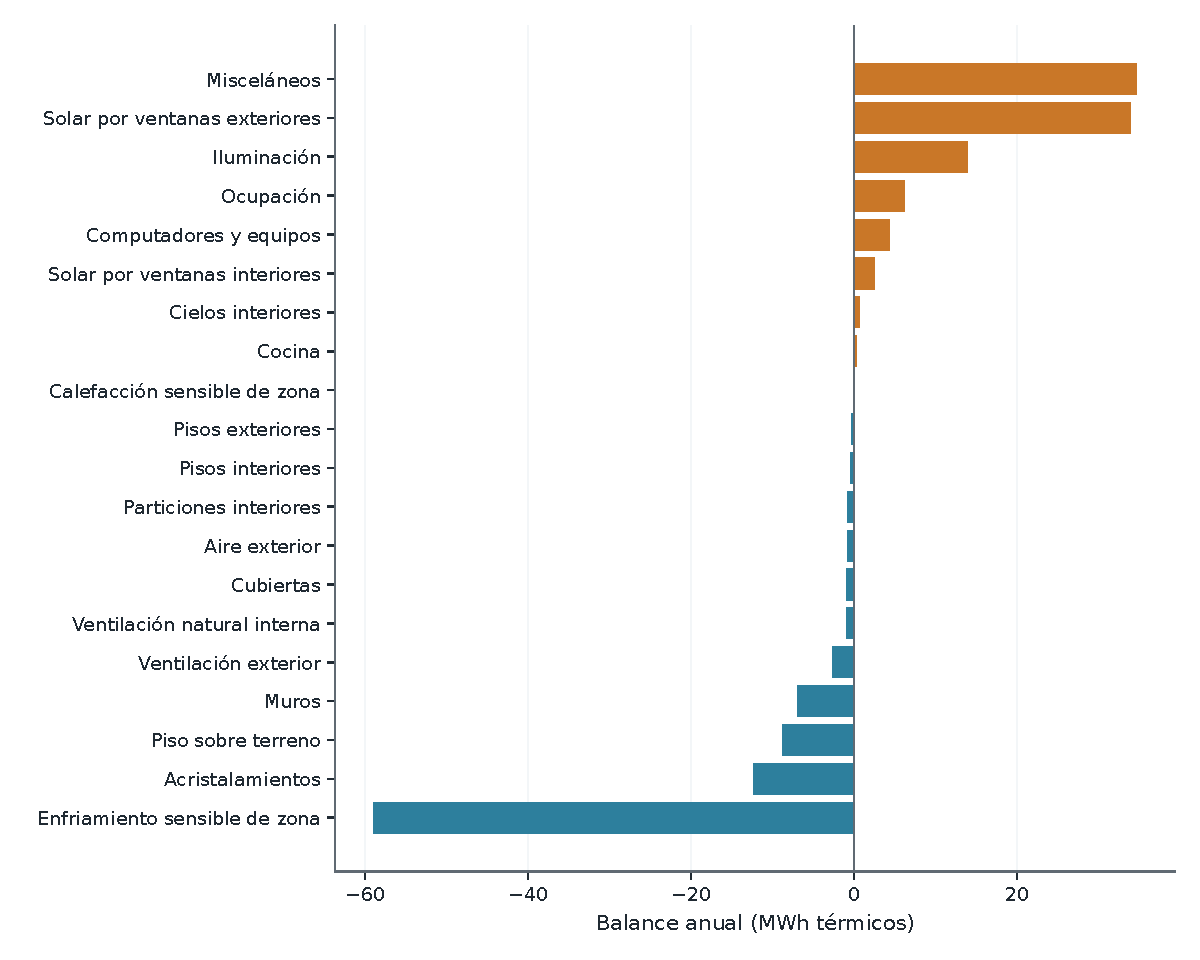
\includegraphics[width=\textwidth]{figuras/caso-base-final-balance-componentes.pdf}
\caption{Balance general anual: aportes y extracciones de calor}
\fuente{Elaboración propia a partir de \texttt{Datos Caso Base3.csv}, exportado de la corrida 09 de DesignBuilder. Resultados provisionales.}
\end{figure}
\clearpage

\begin{figure}[H]
\centering
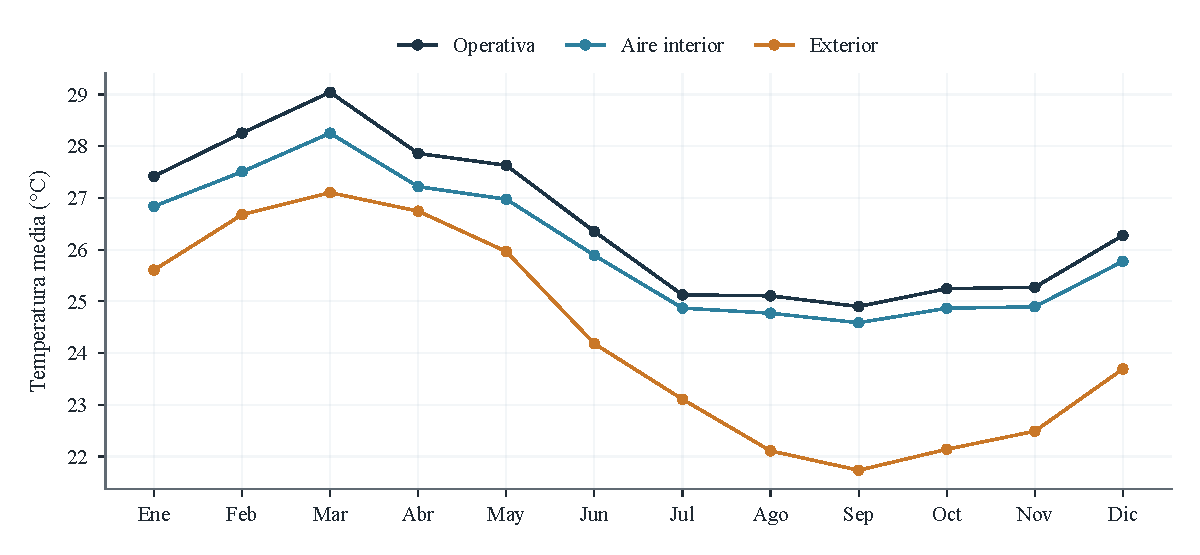
\includegraphics[width=\textwidth]{figuras/caso-base-final-temperatura-mensual.pdf}
\caption{Temperaturas medias mensuales del edificio y del exterior}
\fuente{Elaboración propia a partir de \texttt{Datos Caso Base3.csv}, exportado de la corrida 09 de DesignBuilder. Resultados provisionales.}
\end{figure}

\begin{figure}[H]
\centering
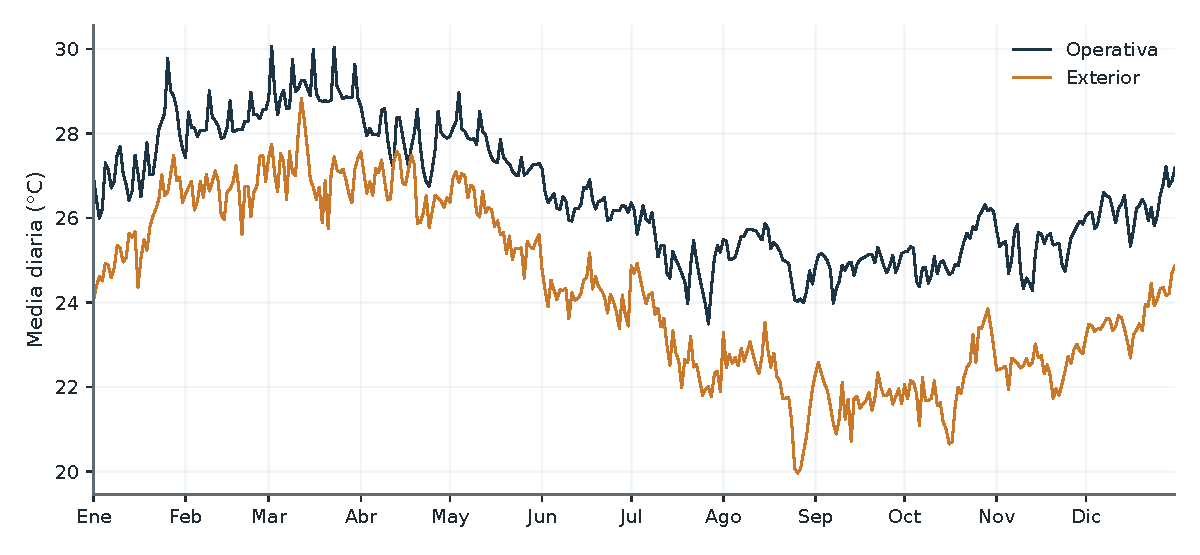
\includegraphics[width=\textwidth]{figuras/caso-base-temperatura-diaria.pdf}
\caption{Evolución de las medias diarias de temperatura}
\fuente{Elaboración propia a partir de \texttt{Datos Caso Base3.csv}, exportado de la corrida 09 de DesignBuilder. Resultados provisionales.}
\end{figure}
\clearpage

\begin{figure}[H]
\centering
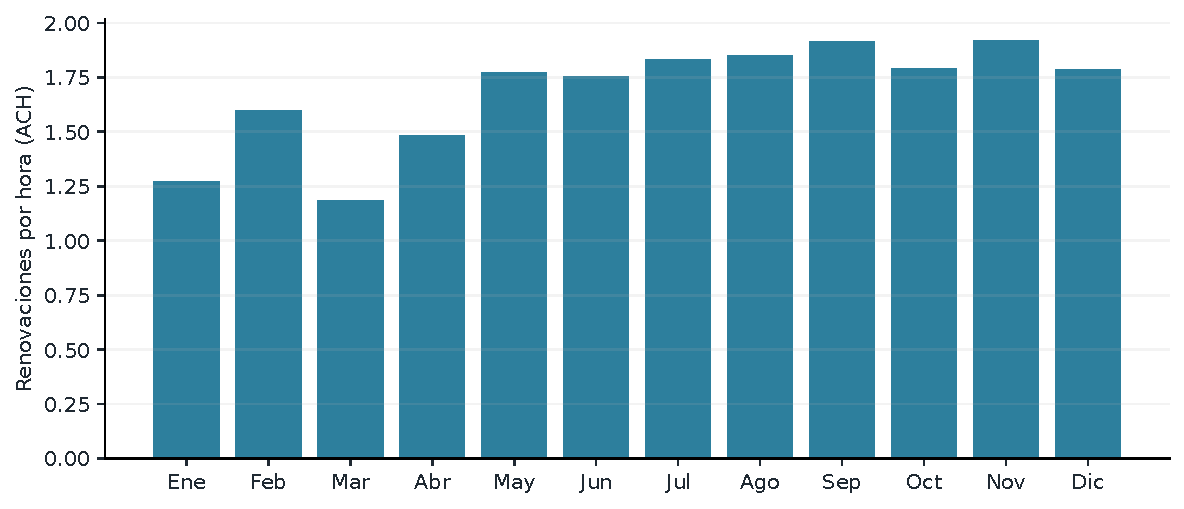
\includegraphics[width=\textwidth]{figuras/caso-base-ventilacion-mensual.pdf}
\caption{Ventilación e infiltración: media mensual del edificio}
\fuente{Elaboración propia a partir de \texttt{Datos Caso Base3.csv}, exportado de la corrida 09 de DesignBuilder. Resultados provisionales.}
\end{figure}

\begin{figure}[H]
\centering
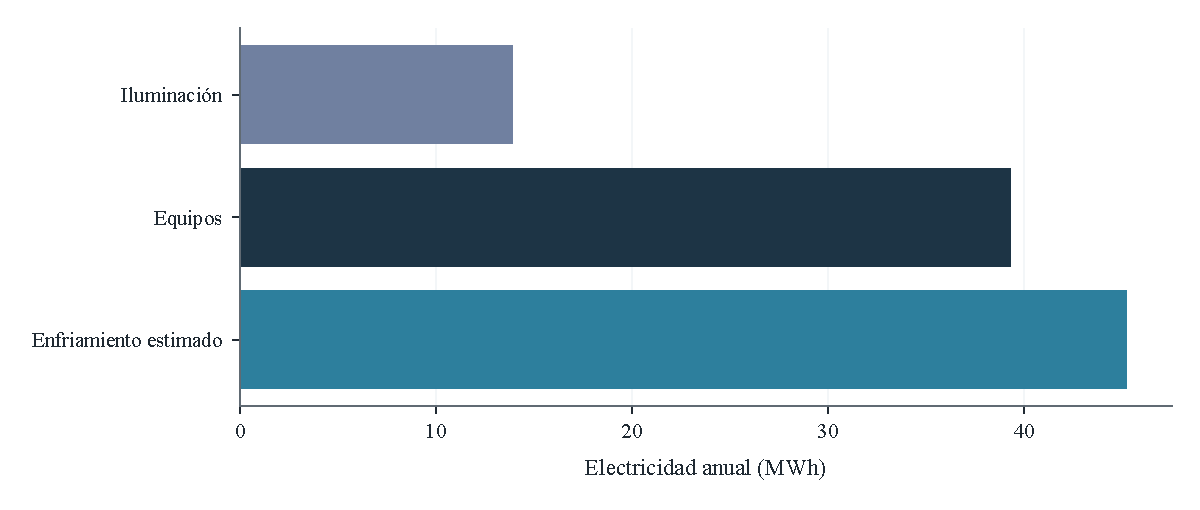
\includegraphics[width=\textwidth]{figuras/caso-base-consumos-electricos.pdf}
\caption{Distribución de la electricidad anual estimada}
\fuente{Elaboración propia a partir de \texttt{Datos Caso Base3.csv}, exportado de la corrida 09 de DesignBuilder. Resultados provisionales.}
\end{figure}
